%% ============================================================================
%%  Fig. 1 of "Self-Supervised Graph Neural Networks for Network Intrusion
%%  Detection with Conformal Safety Certification".
%%
%%  Hand-authored TikZ source, NOT AI-generated.
%%  Compile with:  pdflatex fig1_pipeline.tex
%%
%%  This file exists to document the provenance of Fig. 1 in response to
%%  the IEEE Access Reviewer 2 concern (2026-08-11): the figure is
%%  algorithmically drawn from the TikZ primitives below and does not
%%  involve any image-generation model.
%% ============================================================================

\documentclass[tikz,border=6pt]{standalone}

\usepackage{tikz}
\usetikzlibrary{arrows.meta,calc,positioning,fit,shapes.geometric,%
                backgrounds,decorations.pathreplacing}
\usepackage{xcolor}

\definecolor{phaseblue}{RGB}{52,103,179}
\definecolor{phasegreen}{RGB}{77,156,107}
\definecolor{accentorange}{RGB}{215,124,44}
\definecolor{novgold}{RGB}{217,166,33}
\definecolor{softgrey}{RGB}{236,238,243}

\begin{document}

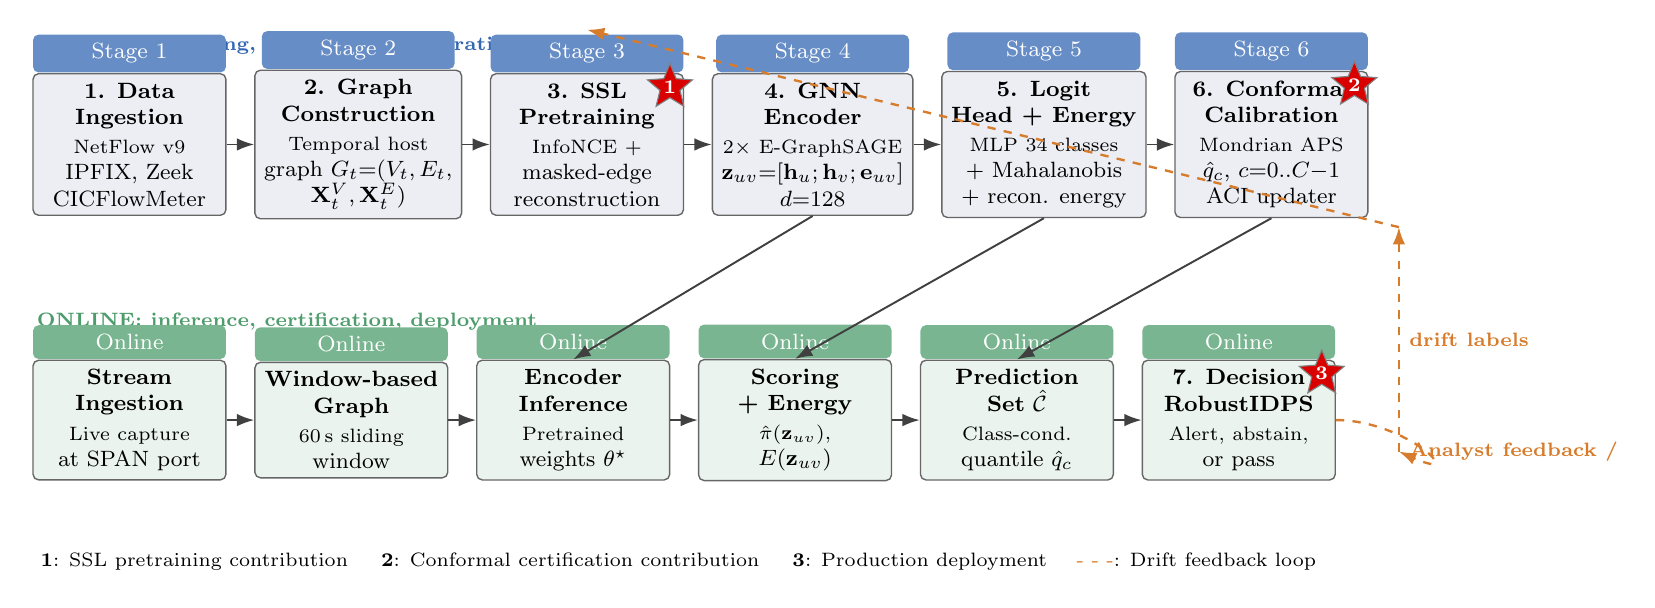
\begin{tikzpicture}[
  font=\footnotesize,
  every node/.style={align=center},
  stage/.style={rounded corners=2pt,draw=black!60,line width=0.5pt,
                minimum width=2.45cm,minimum height=1.35cm,fill=softgrey},
  offlineheader/.style={fill=phaseblue!75,text=white,
                rounded corners=2pt,minimum width=2.45cm,minimum height=0.35cm},
  onlineheader/.style={fill=phasegreen!75,text=white,
                rounded corners=2pt,minimum width=2.45cm,minimum height=0.35cm},
  novbadge/.style={star,star points=5,star point ratio=2.25,
                fill=red!85!black,draw=black!50,inner sep=0pt,
                minimum size=0.6cm,text=white,font=\scriptsize\bfseries},
  flow/.style={-{Latex[length=2.2mm,width=1.6mm]},line width=0.7pt,black!75},
  feedback/.style={-{Latex[length=2.2mm,width=1.6mm]},line width=0.85pt,
                dashed,accentorange}
]

% Phase band labels
\node[anchor=west] (offlbl) at (-0.6,1.95)
  {\scriptsize\textbf{\color{phaseblue}OFFLINE: training, pretraining, calibration}};
\node[anchor=west] (onlbl) at (-0.6,-1.55)
  {\scriptsize\textbf{\color{phasegreen}ONLINE: inference, certification, deployment}};

% --- Offline (top) row ---
\node[stage] (s1) at (0.7,0.7)
  {\textbf{1. Data}\\\textbf{Ingestion}\\[1pt]
   \scriptsize NetFlow v9\\IPFIX, Zeek\\CICFlowMeter};
\node[offlineheader,above=0pt of s1.north] {Stage 1};

\node[stage,right=0.35cm of s1] (s2)
  {\textbf{2. Graph}\\\textbf{Construction}\\[1pt]
   \scriptsize Temporal host\\graph $G_t{=}(V_t,E_t,$\\$\mathbf{X}_t^V,\mathbf{X}_t^E)$};
\node[offlineheader,above=0pt of s2.north] {Stage 2};

\node[stage,right=0.35cm of s2] (s3)
  {\textbf{3. SSL}\\\textbf{Pretraining}\\[1pt]
   \scriptsize InfoNCE +\\masked-edge\\reconstruction};
\node[offlineheader,above=0pt of s3.north] {Stage 3};
\node[novbadge] at ($(s3.north east)+(-0.18,-0.18)$) {1};

\node[stage,right=0.35cm of s3] (s4)
  {\textbf{4. GNN}\\\textbf{Encoder}\\[1pt]
   \scriptsize 2$\times$ E-GraphSAGE\\$\mathbf{z}_{uv}{=}[\mathbf{h}_u;\mathbf{h}_v;\mathbf{e}_{uv}]$\\$d{=}128$};
\node[offlineheader,above=0pt of s4.north] {Stage 4};

\node[stage,right=0.35cm of s4] (s5)
  {\textbf{5. Logit}\\\textbf{Head + Energy}\\[1pt]
   \scriptsize MLP $34$ classes\\$+$ Mahalanobis\\$+$ recon. energy};
\node[offlineheader,above=0pt of s5.north] {Stage 5};

\node[stage,right=0.35cm of s5] (s6)
  {\textbf{6. Conformal}\\\textbf{Calibration}\\[1pt]
   \scriptsize Mondrian APS\\$\hat{q}_c$, $c{=}0..C{-}1$\\ACI updater};
\node[offlineheader,above=0pt of s6.north] {Stage 6};
\node[novbadge] at ($(s6.north east)+(-0.18,-0.18)$) {2};

% --- Online (bottom) row ---
\node[stage,fill=phasegreen!12] (o1) at (0.7,-2.8)
  {\textbf{Stream}\\\textbf{Ingestion}\\[1pt]
   \scriptsize Live capture\\at SPAN port};
\node[onlineheader,above=0pt of o1.north] {Online};

\node[stage,fill=phasegreen!12,right=0.35cm of o1] (o2)
  {\textbf{Window-based}\\\textbf{Graph}\\[1pt]
   \scriptsize 60\,s sliding\\window};
\node[onlineheader,above=0pt of o2.north] {Online};

\node[stage,fill=phasegreen!12,right=0.35cm of o2] (o3)
  {\textbf{Encoder}\\\textbf{Inference}\\[1pt]
   \scriptsize Pretrained\\weights $\theta^\star$};
\node[onlineheader,above=0pt of o3.north] {Online};

\node[stage,fill=phasegreen!12,right=0.35cm of o3] (o4)
  {\textbf{Scoring}\\\textbf{+ Energy}\\[1pt]
   \scriptsize $\hat{\pi}(\mathbf{z}_{uv})$,\\$E(\mathbf{z}_{uv})$};
\node[onlineheader,above=0pt of o4.north] {Online};

\node[stage,fill=phasegreen!12,right=0.35cm of o4] (o5)
  {\textbf{Prediction}\\\textbf{Set} $\hat{\mathcal{C}}$\\[1pt]
   \scriptsize Class-cond.\\quantile $\hat{q}_c$};
\node[onlineheader,above=0pt of o5.north] {Online};

\node[stage,fill=phasegreen!12,right=0.35cm of o5] (o6)
  {\textbf{7. Decision}\\\textbf{RobustIDPS}\\[1pt]
   \scriptsize Alert, abstain,\\or pass};
\node[onlineheader,above=0pt of o6.north] {Online};
\node[novbadge] at ($(o6.north east)+(-0.18,-0.18)$) {3};

% --- Horizontal forward arrows ---
\draw[flow] (s1) -- (s2);
\draw[flow] (s2) -- (s3);
\draw[flow] (s3) -- (s4);
\draw[flow] (s4) -- (s5);
\draw[flow] (s5) -- (s6);
\draw[flow] (o1) -- (o2);
\draw[flow] (o2) -- (o3);
\draw[flow] (o3) -- (o4);
\draw[flow] (o4) -- (o5);
\draw[flow] (o5) -- (o6);

% --- Vertical hand-off arrows from offline to online stages ---
\draw[flow] (s4.south) -- (o3.north);
\draw[flow] (s5.south) -- (o4.north);
\draw[flow] (s6.south) -- (o5.north);

% --- Feedback loop ---
\draw[feedback]
  (o6.east) .. controls +(0.9,0) and +(0.9,-0.4) ..
  ++(0.8,-0.4) node[right,font=\scriptsize\bfseries,text=accentorange]
  {Analyst feedback /};
\draw[feedback] ($(o6.east)+(0.8,-0.4)$) -- ++(0,2.85)
  node[midway,right,font=\scriptsize\bfseries,text=accentorange]{drift labels};
\draw[feedback]
  ($(o6.east)+(0.8,2.45)$) -- ($(s3.north)+(0,0.55)$);

% --- Legend ---
\node[anchor=west,font=\scriptsize] at (-0.6,-4.6)
  {\textcolor{red!85!black}{$\bigstar$}\,\textbf{1}: SSL pretraining contribution \quad
   \textcolor{red!85!black}{$\bigstar$}\,\textbf{2}: Conformal certification contribution \quad
   \textcolor{red!85!black}{$\bigstar$}\,\textbf{3}: Production deployment \quad
   \textcolor{accentorange}{- - -}: Drift feedback loop};

\end{tikzpicture}

\end{document}
